Die Benutzeroberfläche einer solch einfachen To-Do-Anwendung besteht aus einer Ansicht. Diese Ansicht lässt sich hierarchisch definieren. Die oberste Ebene dieser Hierarchie bildet der hier sog. \textit{App-Container}. Anders als in aufwändigeren Applikationen kann dieser hier mit der Ansicht gleichgesetzt werden, da keine weiteren Ansichten existieren. Dieser Container beherbergt eine Listenansicht, welche für die Darstellung und Interaktion mit den bereits vorhandenen Einträgen zuständig ist. Für das Erstellen der Einträge steht ein separates Text(eingabe)feld zur Verfügung, sowie ein \textit{Button} zur Bestätigung der Eingabe.

Die Listenansicht besteht nun aus mehreren Listeneinträgen (im Folgenden \texttt{Zellen} genannt). Eine Zelle ist für die Darstellung und Interaktion für genau einen To-Do-Eintrag zuständig. Um dies zu ermöglichen, besitzt jede Zelle, neben eines Textfeldes zum Anzeigen des To-Do-Textes, weitere Buttons zum Setzen der Priorität und des Status sowie zum Löschen des Eintrages. Während der Button, welcher für das Entfernen des Eintrages verwendet wird (dargestellt durch ein Kreuz, statischer optischer Natur ist (d.\ h., er ändert nach einem Tippen sein Aussehen nicht), untermalen die Buttons der To-Do-Zustände die gewählten Einstellungen durch ihr Aussehen. Der Button für Priorisierung, welcher durch ein Sternsymbol dargestellt wird, ist bei aktiver Priorisierung gefüllt. Ist dies nicht der Fall, so ist lediglich der Umriss des Symbols zu erkennen. Gleiches gilt für den Button, welcher anzeigt, ob der Eintrag bereits erledigt ist, dargestellt durch ein Häkchen inmitten eines Kreises.

Die beschriebenen, visuellen Eigenschaften lassen sich nun in einem sog. \textit{Wireframe} zusammenfassen, welches gleichzeitig die optische Grundlage der Entwicklung darstellen wird. Dies ist vor allem aufgrund der unterschiedlichen Entwicklungsplattformen von Relevanz, da das Einhalten bestimmter Standards der entsprechenden Plattformen dafür sorgen könnte, dass der letztendliche Vergleich beider Applikationen hohe Differenzen aufweist. Das Wireframe ist in Abb. \ref{fig:wireframe} abgebildet.

\begin{figure}[h!]
	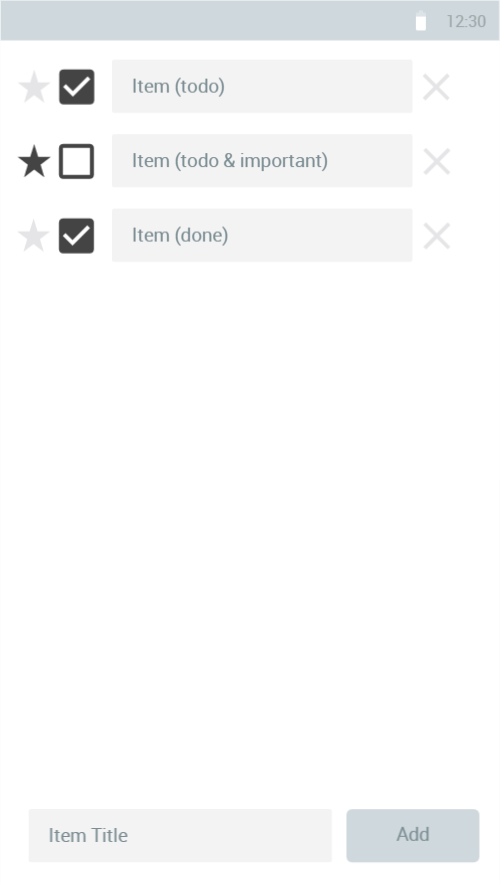
\includegraphics[scale=0.5]{img/fig/4-3-1_wireframe.png}
	\centering
	\caption{Wireframe der App}
	\label{fig:wireframe}
\end{figure}

Eine Besonderheit in der Darstellung lässt sich innerhalb der priorisierten Elemente finden. Um diese weiter hervorzuheben, werden diese an den Anfang der Liste gesetzt. Es entstehen somit zwei Teillisten, welche sich jedoch in derselben Listenansicht befinden. Wird nun ein zuvor nicht-priorisierter Eintrag priorisiert, so wechselt dieser seine Position ans Ende der Liste mit den bereits priorisierten Einträgen (bzw. wird oberhalb der ersten nicht-priorisierten Elements platziert). Alle Einträge zwischen der alten und der neuen Position des gerade betrachteten Eintrags werden um eine Listenposition nach unten verschoben. Bei Entfernen der Priorisierung wird das entsprechende Element nun nicht an seine ursprüngliche Position vor der Priorisierung, sondern an den Anfang der nicht-priorisierten Liste verschoben. Entfernt man also bspw. die Priorisierung des letzten Elements in der priorisierten Liste, ändert sich die Reihenfolge nicht. Dieses Verhalten kann vereinfacht in der untenstehenden Abbildung dargestellt werden.

Grundsätzlich werden alle Einträge in der Reihenfolge dargestellt, wie sie angelegt wurden, mit den eben beschriebenen Ausnahmen.

Um ebenfalls für farbliche Konsistenz zu sorgen, werden die beschriebenen Elemente auf Basis der folgenden Tabelle in ihrem Erscheinungsbild konfiguriert:

\begin{table}[h!]
	\centering
	\begin{tabular}{ |c|c|c|}
		\hline
		\textbf{Bezeichnung} & \textbf{Hex-Code} & \textbf{Darstellung}\\
		\hline
		
		
		\hline
		\multicolumn{3}{|c|}{\textbf{Allgemeines}}\\
		\hline
		Hintergrund & \texttt{\#F2F2F2} &\cellcolor[HTML]{F2F2F2}\\
		\hline
		Schriftfarbe & \texttt{\#8C8C8C} &\cellcolor[HTML]{8C8C8C}\\
		\hline
		
		
		\hline
		\multicolumn{3}{|c|}{\textbf{Bedienelemente}}\\
		\hline
		Hintergrund für inaktive Bedienelemente & \texttt{\#CECECE} &\cellcolor[HTML]{CECECE}\\
		\hline
		Hintergrund der Checkbox (angewählt) & \texttt{\#1A66FF} &\cellcolor[HTML]{1A66FF}\\
		\hline
		Schriftfarbe der Checkbox (angewählt) & \texttt{\#FFFFFF} &\cellcolor[HTML]{FFFFFF}\\
		\hline
	\end{tabular}
	\caption{Farbtabelle} \label{tab:farbtabelle}
\end{table}
